\documentclass{article}

\usepackage{graphicx}
\usepackage{tikz}
\usepackage{tikzsymbols}
\usetikzlibrary{calc,patterns,shapes.geometric}
\pagestyle{empty}
\usepackage[margin=0pt]{geometry}
\geometry{papersize={14in,12in}}

\def\centerarc[#1](#2)(#3:#4:#5){\draw[#1] ($(#2)+({#5*cos(#3)},{#5*sin(#3)})$) arc (#3:#4:#5);}

\begin{document}
	\begin{figure}
		\centering
		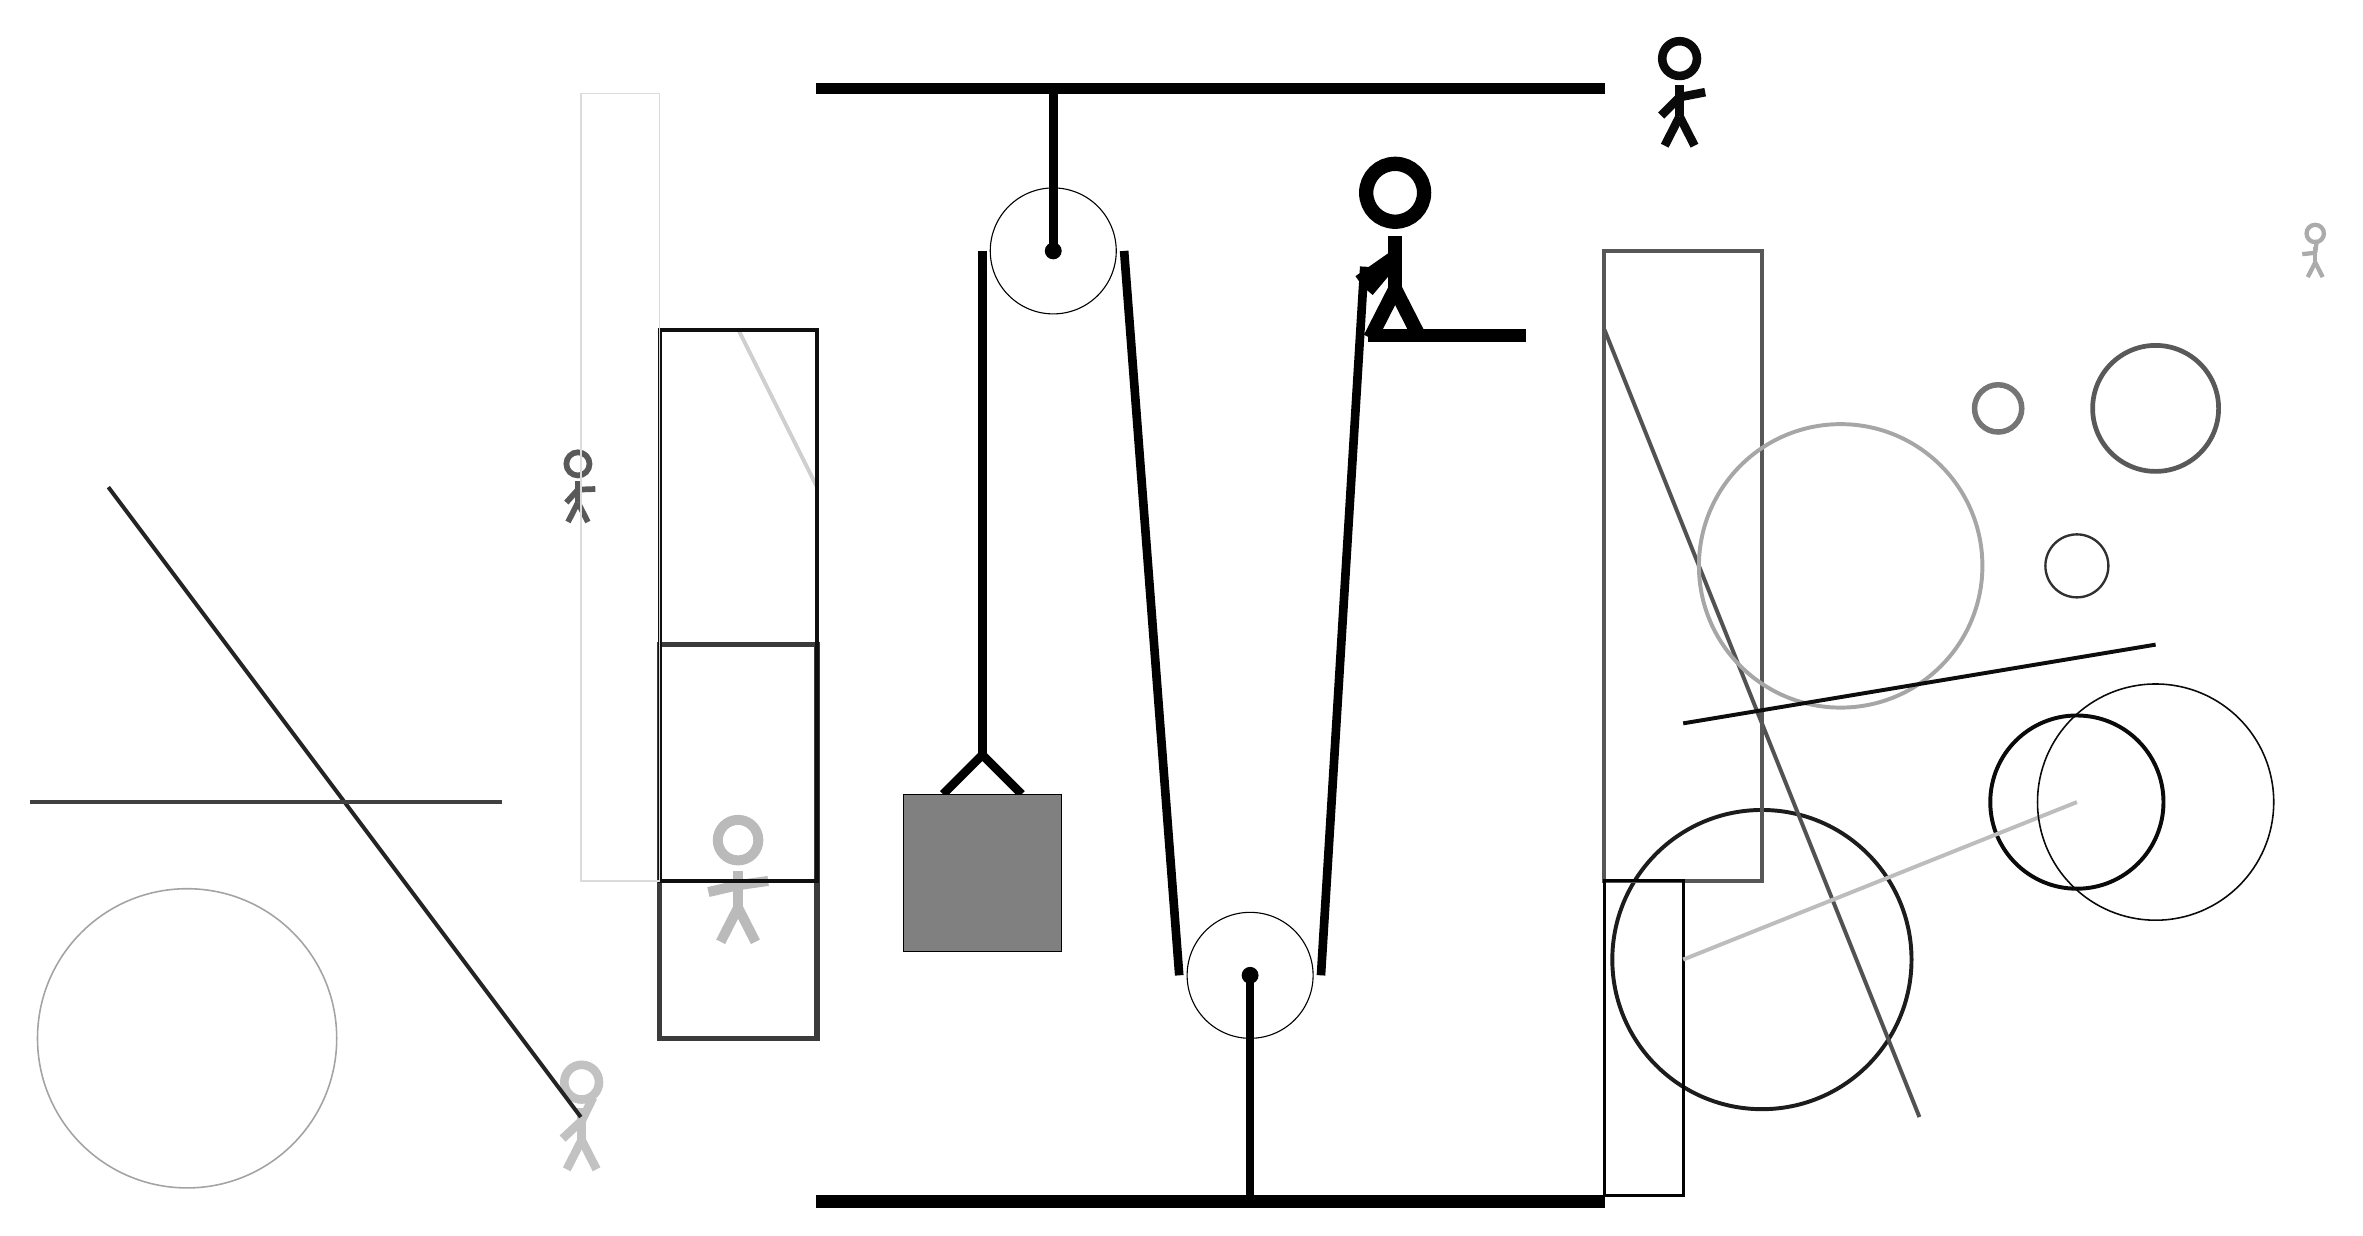
\begin{tikzpicture}
			%%%%% START %%%%%
			
			\draw[fill=black] (-2, 14) rectangle (8, 14.125);
			
			\node[line width=0.7mm, color=black!27] at (-3, 4) {\Strichmaxerl[7][13][8]};
			
			\draw [line width=0.5mm, color=black!59](10, 7) circle (0.0);
			\draw [line width=0.5mm, color=black!89](10, 3) circle (1.9);
			\node[line width=0.2mm, color=black!96] at (9, 14) {\Strichmaxerl[6][45][11]};
			\draw[line width=0.5mm, color=black!68](8, 11) -- (12, 1);
			\draw[line width=0.5mm, color=black!66] (8, 4) rectangle (10, 12);
			\draw[line width=0.4mm, color=black!99] (8, 0) rectangle (9, 4);
			
			\node[line width=0.5mm, color=black!24] at (-5, 1) {\Strichmaxerl[6][43][64]};
			\draw[line width=0.7mm, color=black!77] (-2, 2) rectangle (-4, 7);
			
			\draw [line width=0.2mm, color=black!36](-10, 2) circle (1.9);
			
			\draw[line width=0.5mm, color=black!86](-5, 1) -- (-11, 9);
			\node[line width=0.5mm, color=black!33] at (17, 12) {\Strichmaxerl[3][6][83]};
			\draw [line width=0.7mm, color=black!69](17, 4) circle (0.0);
			
			\draw [line width=0.6mm, color=black!65](15, 10) circle (0.8);
			\draw[line width=0.5mm, color=black!19](-3, 11) -- (-2, 9);
			\draw [line width=0.5mm, color=black!96](14, 5) circle (1.1);
			
			\draw [line width=0.5mm, color=black!35](11, 8) circle (1.8);
			
			\node[line width=0.7mm, color=black!65] at (-5, 9) {\Strichmaxerl[4][48][2]};
			\draw[line width=0.5mm, color=black!94] (-2, 4) rectangle (-4, 11);
			
			\draw [line width=0.7mm, color=black!54](13, 10) circle (0.3);
			\draw[line width=0.5mm, color=black!95](9, 6) -- (15, 7);
			
			\draw[line width=0.5mm, color=black!26](9, 3) -- (14, 5);
			\draw[line width=0.2mm, color=black!14] (-4, 14) rectangle (-5, 4);
			\draw [line width=0.3mm, color=black!81](14, 8) circle (0.4);
			\draw [line width=0.2mm, color=black!96](15, 5) circle (1.5);
			
			\draw[line width=0.5mm, color=black!75](-6, 5) -- (-12, 5);
			
			\draw (3.5, 2.8) circle (0.8);
			\draw[fill=black] (3.5, 2.8) circle (0.1);
			\draw[line width=1.1mm] (3.5, 2.8) -- (3.5, 0);
			
			\draw (1, 12) circle (0.8);
			\draw[fill=black] (1, 12) circle (0.1);
			\draw[line width=1.1mm] (1, 14) -- (1, 12);
			
			\draw[line width=1.1mm](-0.4, 5.1) --  (0.1, 5.6) -- (0.6, 5.1);
			\draw[fill=black!50] (-0.9, 5.1) rectangle (1.1, 3.1);
			
			\draw[line width=1.1mm](0.1, 12) -- (0.1, 5.6);
			\centerarc[line width=1.1mm](1, 12)(180:0:0.9)
			\draw[line width=1.1mm](1.9, 12) -- (2.6, 2.8);
			\centerarc[line width=1.1mm](3.5, 2.8)(180:360:0.9)
			\draw[line width=1.1mm](4.4, 2.8) -- (4.95, 11.8);
			
			\node at (5.3, 12) {\Strichmaxerl[10][35][-130]};
			\draw[fill=black] (5, 11) rectangle (7, 10.85);
			
			\draw[fill=black] (-2, 0) rectangle (8, -0.15);
			
			%%%%% END %%%%%
		\end{tikzpicture}
	\end{figure}	
\end{document}